Use ifelse  for the following
\begin{enumerate}[label=\thesubsection.\arabic*, ref=\thesubsection.\theenumi]
	\item $25 \times \brak{-21} = \brak{-21}\times 25 $
	\\
	\solution 
	\lstinputlisting{codes/prog/compeq.c}
	\begin{multicols}{2}
	\item $\brak{-48}\div\brak{8} = 48 \div \brak{-8}$
	\item $\brak{-23}\times  20 = 23 \times \brak{-20}$
	\item $90 \div \brak{-45} = \brak{-90}\div 45$
	\item $ \brak{-136}\div 4=136 \div \brak{-4} $
	\item $10\times  \sbrak{6+\brak{-2}} =10\times 6+10 \times \brak{-2} $
	\item $10\times  \sbrak{6-\brak{-2}} =10\times 6-10 \times \brak{-2} $
\end{multicols}
	\item $\brak{-15}\times  \sbrak{\brak{-7}-\brak{-1}} =\brak{-15}\times\brak{-7}-\brak{-15} \times \brak{-1} $
	\item $18\times  \sbrak{\brak{7}+\brak{-3}} =18\times\brak{7}+18 \times \brak{-3} $
	\item $\brak{-21}\times  \sbrak{\brak{-4}+\brak{-6}} =\brak{-21}\times\brak{-4}+\brak{-21} \times \brak{-6} $
	\item $\brak{-15}\times  \sbrak{\brak{-7}+\brak{-1}} =\brak{-15}\times\brak{-7}+\brak{-15} \times \brak{-1} $
\end{enumerate}
\begin{enumerate}[label=\thesubsection.\arabic*, ref=\thesubsection.\theenumi,resume*]
	\item 		An angle is greater than 45\degree. Is its complementary angle greater than 45\degree or equal to 45\degree or less than 45\degree?
\end{enumerate}
	Is it possible to have a triangle with the following sides? 
\begin{enumerate}[label=\thesubsection.\arabic*, ref=\thesubsection.\theenumi,resume*]
		\begin{multicols}{2}
\item $2 cm, 3 cm, 5 cm $ 
\item $3 cm, 6 cm, 7 cm $
\item $ 6 cm, 3 cm, 2 cm$
\item $10.2 cm, 5.8 cm, 4.5 cm$?
\end{multicols}
	\end{enumerate}
	 Between which two numbers can length of the third side fall?
	The lengths of two sides of a triangle are 
\begin{enumerate}[label=\thesubsection.\arabic*, ref=\thesubsection.\theenumi,resume*]
	\begin{multicols}{2}
		\item $6 cm$ and $8 cm$.
		\item $12 cm$ and $15 cm$.
		\end{multicols}
	\end{enumerate}
Which is greater?
\begin{enumerate}[label=\thesubsection.\arabic*, ref=\thesubsection.\theenumi,resume*,itemsep=1ex]
	\begin{multicols}{2}
	\item $\frac{1}{2}$ of $\frac{3}{4}$
	or $\frac{3}{5}$ of $\frac{5}{8}$
	\item $\frac{1}{2}$ of $\frac{6}{7}$
	or $\frac{2}{3}$ of $\frac{3}{7}$
\end{multicols}
\end{enumerate}
Identify which of the following pairs of angles are complementary and which are supplementary.
\begin{enumerate}[label=\thesubsection.\arabic*, ref=\thesubsection.\theenumi,resume*]
	\begin{multicols}{4}
	\item  65\degree, 115\degree
	\item  63\degree, 27\degree 
	\item  130\degree, 50\degree 
	\item 45\degree, 45\degree 
	\item  112\degree, 68\degree 
	\item  80\degree, 10\degree
\end{multicols}
\end{enumerate}
Which of these are negative rational numbers?
\begin{enumerate}[label=\thesubsection.\arabic*, ref=\thesubsection.\theenumi,resume*,itemsep=1ex]
	\begin{multicols}{4}
	\item $\frac{-2}{3}$
	\item $\frac{5}{7}$
	\item $\frac{3}{-5}$
	\item $\frac{6}{11}$
	\item $\frac{-2}{-9}$
	\item 0
\end{multicols}
\end{enumerate}
Compare the following and fill in the blanks
\begin{enumerate}[label=\thesubsection.\arabic*, ref=\thesubsection.\theenumi,resume*,itemsep=1ex]
	\begin{multicols}{4}
		\item $\frac{-5}{7} \rule{0.5cm}{0.1pt} \frac{2}{3}$
		\item $\frac{-8}{5} \rule{0.5cm}{0.1pt} \frac{-7}{4}$
		\item ${0} \rule{0.5cm}{0.1pt} \frac{-7}{6}$
		\item $\frac{-4}{5} \rule{0.5cm}{0.1pt} \frac{-5}{7}$
		\item $\frac{1}{-3} \rule{0.5cm}{0.1pt} \frac{-1}{4}$
		\item $\frac{-7}{8} \rule{0.5cm}{0.1pt} \frac{14}{-16}$
		\item $\frac{5}{-11} \rule{0.5cm}{0.1pt} \frac{-5}{11}$
		\item $\frac{2}{3} \rule{0.5cm}{0.1pt} \frac{5}{7}$
		\item $\frac{-3}{8} \rule{0.5cm}{0.1pt} \frac{-2}{7}$
		\item $\frac{-4}{3} \rule{0.5cm}{0.1pt} \frac{-3}{2}$
		\item $\frac{-7}{21} \rule{0.5cm}{0.1pt} \frac{3}{9}$
		\item $\frac{-3}{5} \rule{0.5cm}{0.1pt} \frac{-12}{20}$
		\item $\frac{-5}{-9} \rule{0.5cm}{0.1pt} \frac{5}{-9}$
		\item $\frac{-16}{20} \rule{0.5cm}{0.1pt} \frac{20}{-25}$
		\item $\frac{8}{-5} \rule{0.5cm}{0.1pt} \frac{-24}{15}$
		\item $\frac{-2}{-3} \rule{0.5cm}{0.1pt} \frac{2}{3}$
		\item $\frac{1}{3} \rule{0.5cm}{0.1pt} \frac{-1}{9}$
		\item $\frac{4}{-9} \rule{0.5cm}{0.1pt} \frac{-16}{36}$
		\item $\frac{2}{3} \rule{0.5cm}{0.1pt} \frac{5}{2}$
		\item $\frac{-1}{4} \rule{0.5cm}{0.1pt} \frac{1}{4}$
		\item $\frac{-5}{6} \rule{0.5cm}{0.1pt} \frac{-4}{3}$
		\item $-3\frac{2}{7} \rule{0.5cm}{0.1pt} -3\frac{4}{5}$
		\item $\frac{-3}{4} \rule{0.5cm}{0.1pt} \frac{2}{-3}$
\end{multicols}
\end{enumerate}
		Write four more numbers in the following pattern
\begin{enumerate}[label=\thesubsection.\arabic*, ref=\thesubsection.\theenumi,resume*,itemsep=1ex]
	\item $\frac{-1}{3},\frac{-2}{6},\frac{-3}{9},\frac{-4}{12}$
		\\
		\solution
	\lstinputlisting{codes/prog/seq.c}
	\begin{multicols}{3}
	\item $\frac{-3}{5},\frac{-6}{10},\frac{-9}{15},\frac{-12}{20}$
	\item $\frac{-1}{4},\frac{-2}{8},\frac{-3}{12}$
	\item $\frac{-1}{6},\frac{2}{-12},\frac{3}{-18},\frac{4}{-24}$
	\item $\frac{-2}{3},\frac{2}{-3},\frac{4}{-6},\frac{6}{-9}$
\end{multicols}
		\end{enumerate}
Reduce to standard form
\begin{enumerate}[label=\thesubsection.\arabic*, ref=\thesubsection.\theenumi,resume*,itemsep=1ex]
	\begin{multicols}{4}
	\item $\frac{36}{-24}$
	\item $\frac{-3}{-15}$
	\item $\frac{-18}{45}$
	\item $\frac{-12}{18}$
	\item $\frac{-8}{6}$
	\item $\frac{25}{45}$
	\item $\frac{-44}{72}$
	\item $\frac{-8}{10}$
\end{multicols}
\end{enumerate}
Use recursion for the following
\begin{enumerate}[label=\thesubsection.\arabic*, ref=\thesubsection.\theenumi,resume*]
	\item $\brak{-1}\times\brak{-2} \times \brak{-3} \times \brak{-4}$ 
		\\
		\solution In this case,
			\begin{align}
					x(n) = -nx(n-1), x(0) = 1 
			\end{align}
			Complete the code using the above equation.
	\begin{multicols}{4}
		\item $2^6$   
		\item $11^2$
		\item $5^4$
		\item $\brak{6^2}^{4}$
		\item $\brak{2^2}^{100}$
		\item $\brak{7^{50}}^{2}$
		\item $\brak{5^3}^{7}$
		\item ${2}^{5}\times {2}^{3}$
		\item ${4}^{3}\times {4}^{2}$
		\item ${5}^{3}\times {5}^{7}\times {5}^{12}$
		\item ${2}^{8}\div{2}^{3}$
		\item ${9}^{11}\div{9}^{7}$
		\item ${7}^{13}\div{7}^{10}$
		\item ${10}^{8}\div{10}^{4}$
		\item ${20}^{15}\div{20}^{13}$
		\item $\brak{-4}^{3}$
		\item $\brak{\frac{3}{5}}^{4}$
		\item $\brak{\frac{-4}{7}}^{5}$
		\item $\brak{-4}^{100}\times \brak{-4}^{20}$
		\end{multicols}
\end{enumerate}
Use arrays for the following
\begin{enumerate}[label=\thesubsection.\arabic*, ref=\thesubsection.\theenumi,resume*]
	\item $\brak{-12}\times  \brak{-11}\times \brak{10} $
		\\
		\solution The product can be expressed as
		\begin{align}
			y = \prod_{k=0}^{2}a_k
		\end{align}
		where
		\begin{align}
			\vec{a} = \myvec{-12 \\ -11 \\ 10}
		\end{align}
	The following code implements this
	\lstinputlisting{codes/prog/prodvec.c}
	\begin{multicols}{3}
	\item $\brak{9}\times\brak{-3} \times \brak{-6}$ 
	\item $\brak{-18}\times\brak{-5} \times \brak{-4}$ 
	\item $\brak{-3}\times\brak{-6} \times \brak{-2} \times \brak{-1}$ 
\end{multicols}
\end{enumerate}
Use matrices for the following
\begin{enumerate}[label=\thesubsection.\arabic*, ref=\thesubsection.\theenumi,resume*]
\item Among two supplementary angles the measure of the larger angle is $44\degree$  more than the measure of the smaller. Find their measures.
\end{enumerate}
\begin{enumerate}[label=\thesubsection.\arabic*, ref=\thesubsection.\theenumi,resume*]
\item 
	A collection of 10 chips with different colours is given in 
\figref{fig:percent2}.
Extend the table using a C program
to include a column for the percentage of chips of each colour.
\begin{figure}[H]
  \centering
  \begin{subfigure}{0.4\textwidth}
    
\includegraphics[width=\textwidth]{figs/percent2.jpg}
    \caption{Chips}
  \end{subfigure}
  \hfill
  \begin{subfigure}{0.4\textwidth}
    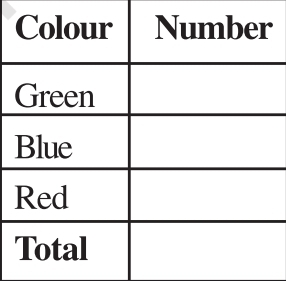
\includegraphics[width=\textwidth]{figs/percent3.jpg}
    \caption{Table}
  \end{subfigure}
  \caption{}
  \label{fig:percent2}
\end{figure}
\end{enumerate}
